\chapter{Literature survey}\label{chap:Lit}

\section{Operational amplifiers}\label{sec:opamps}

\subsubsection{Operational amplifiers: limitations and considerations}\label{sec:opamps_limits}
There are many practical limitations to operational amplifiers in comparison to the ideal model. The limit on the common mode voltage is a concern as the limit is usually around the rail voltage and since the negative rail will be ground and the common mode voltage will be close to 0 the data sheet should be consulted to ensure normal operation of the op amp \cite{NonIdeal_Opamps}. 

A significant consideration is the offset voltage between the inputs of the opamp as when the inputs are equal (no current is being given to the load) there will be an offset voltage on the order of mV which is a similar magnitude to the relevant voltages \cite{Lim_Opamps}. This will result in significant output voltages at no load. However a negative feedback will greatly reduce the impact of input offset voltage and current \cite{Lim_Opamps}.

The output voltage won't be able to go all the way to the rail voltages. Therefore there will be some output voltage when there is no current through the load due to the output not able to go below a certain voltage above ground.
\subsubsection{Operational amplifier configurations}\label{sec:opamps_configs}
There are many different configurations for operational amplifiers, this section will cover 4 basic configurations that could be useful for the current sensor.

The simplest circuit is the voltage follower, it requires no other components and causes the output voltage to track the input voltage. The op amp in this configuration provides a large input impedance and very low output impedance which can allow signals to pass between logic components without them loading each other and can be used to stabilize a voltage divider \cite{Fund_Opamps}.

The inverting op amp is a configuration where the output is connected to the inverting input terminal using a resistor, there is a second resistor connecting this terminal to the circuit input. The non-inverting input is connected to ground. This configuration results in a gain equal to the negative of the ratio between the two resistors. The negative gain cause the output to be exactly out of phase with the input \cite{Fund_Opamps}.

The non-inverting op amp configuration is similar to the inverting amplifier except the input is connected directly to the non-inverting input and the inverting input terminal has a resistor connecting it to the ground. This results in the gain being equal to 1 plus the ratio between the two resistors \cite{Fund_Opamps}.

The differential amplifier is similar to the inverting amplifier, but instead of connecting the non-inverting input to ground a second signal is connected to the input of this terminal through a resistor of the same value  as the other terminal. This results in the output being the difference between the two signals scaled by the ratio of the feedback resistor to the input resistor. This configuration is good at filtering out noise common to both input terminals \cite{Fund_Opamps}. 

\begin{figure}[H]
\footnotesize
\centering
\begin{subfigure}[]{0.45\textwidth}
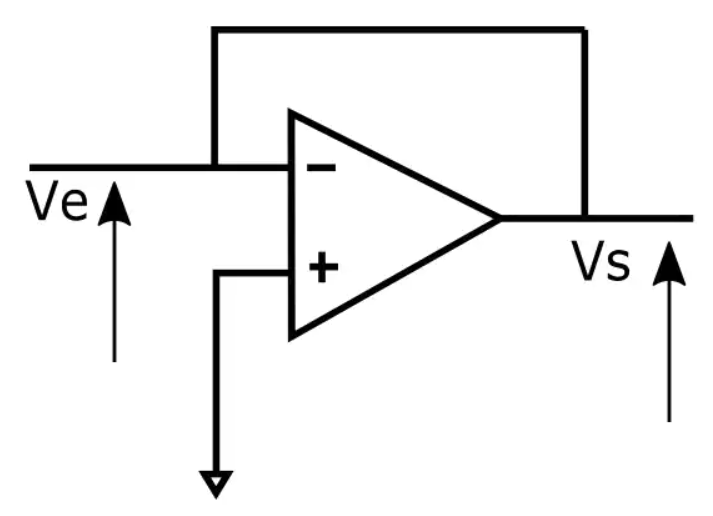
\includegraphics[width=\linewidth]{./Figures/Follower.png}
\caption{Circuit diagram for a voltage follower\cite{Fund_Opamps}}
\label{subfig:opamp_foll}	
\end{subfigure}
\begin{subfigure}[]{0.45\textwidth}
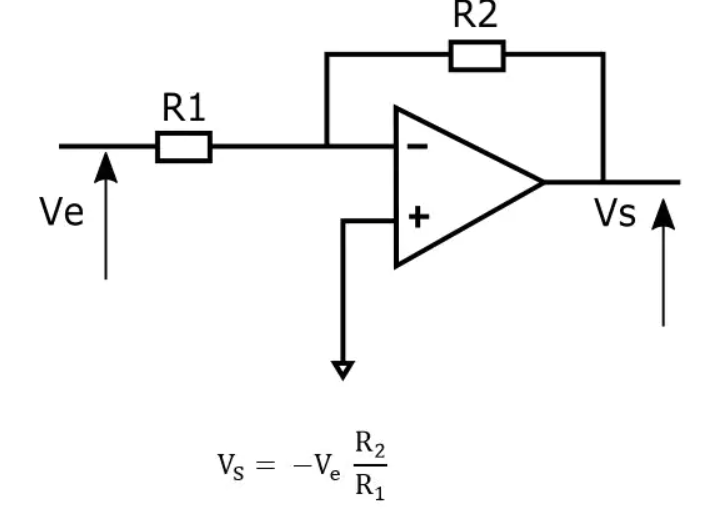
\includegraphics[width=\linewidth]{./Figures/Inverting.png}
\caption{Circuit diagram for a inverting op amp \cite{Fund_Opamps}.} 			
\label{subfig:opamp_invert}	
\end{subfigure}
\begin{subfigure}[]{0.45\textwidth}
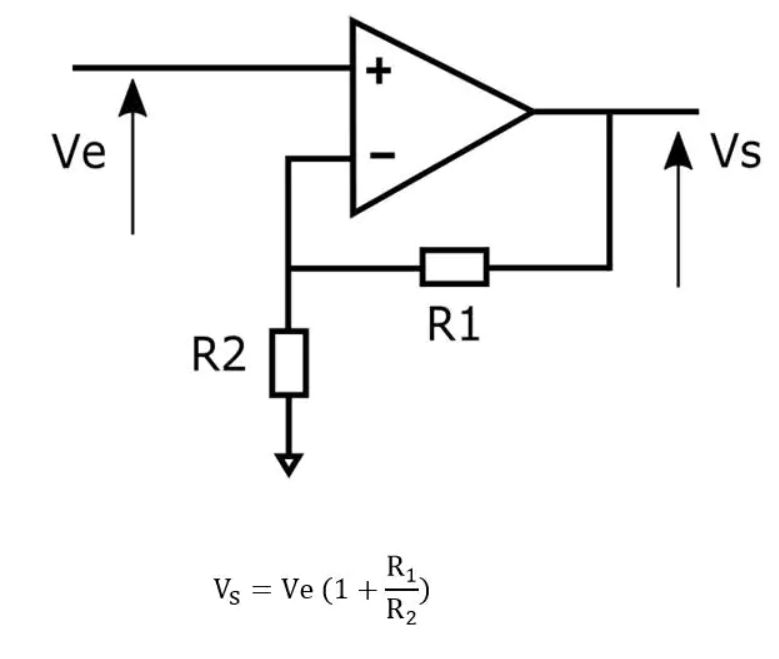
\includegraphics[width=\linewidth]{./Figures/NonInverting.png}
\caption{Circuit diagram for a non-inverting op amp \cite{Fund_Opamps}}
\label{subfig:opamp_noninvert}	
\end{subfigure}
\begin{subfigure}[]{0.45\textwidth}
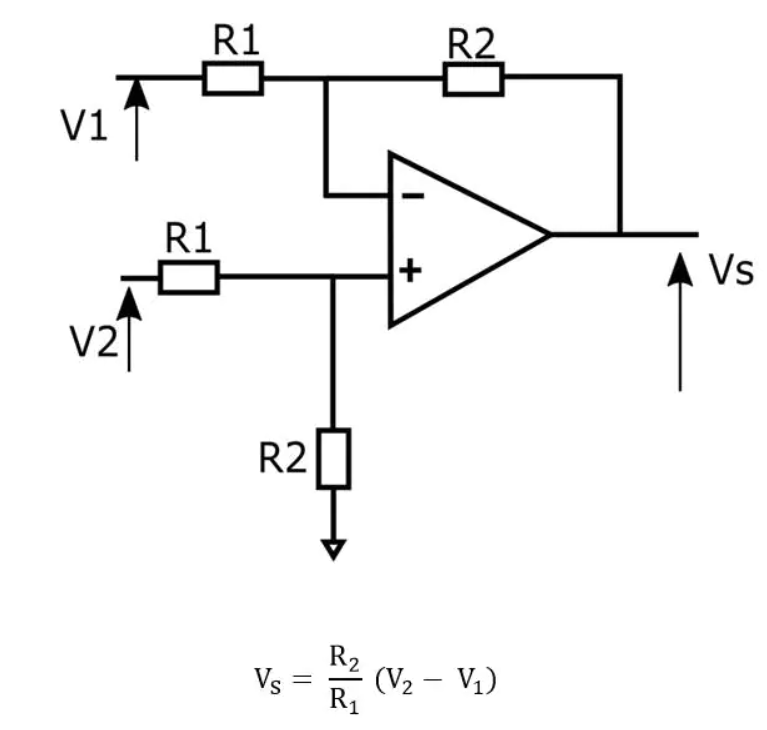
\includegraphics[width=\linewidth]{./Figures/Differential.png}
\caption{Circuit diagram for a differential op amp \cite{Fund_Opamps}} 			
\label{subfig:opamp_dif}	
\end{subfigure}
\caption {Circuit diagrams of 4 op amp configurations}.
\label{fig:circuit_diagram}
\end{figure}

\newpage
\section{Current sensing}\label{sec:cursens}
There are many different techniques to measure current. Both invasive and non invasive methods each with their own advantages and disadvantages that make them suitable for different situations. An invasive current sensor negatively affect the system and decreases performance whereas a non-invasive current sensor doesn't affect the operation of the system at a meaningful level. 

\subsubsection{Hall effect}\label{sec:cursens_hall}
The Hall effect current sensor is a non invasive method of current sensing that uses the magnetic field generated around a current carrying conductor \cite{CircuitDigest}. This magnetic field creates a voltage across the material of the sensor. Hall effect sensors measure this voltage to determine the current flowing in a conductor \cite{Hall}. There are many advantages to using a Hall effect sensor however, besides the amplifier circuit additional circuits are required and is more costly than other measurement methods \cite{CircuitDigest}.

\subsubsection{Rogowski coil}\label{sec:cursens_coil}
The Rogowski coil is a non invasive current sensing method that uses a helical shaped coil that is wrapped around the conductor that you want to measure current in. The coil outputs a voltage depending on the rate of change of current through the conductor, this requires an integrator circuit to create an output voltage that is proportional to the current. The Rogowski coil is very useful for high frequency currents and does not require complex temperature compensation. However this method is only suitable for AC current \cite{CircuitDigest}.

\subsubsection{Shunt Resistor}\label{sec:cursens_shunt}
The shunt resistor is the most common current sensing technique and uses a resistor in series with the current to be measured. This is a invasive current measuring method. The shunt resistor produces a voltage drop proportional to the current, however the resistance and hence the voltage must be kept low in order to reduce the power consumption. This requires a high gain amplifier circuit to increase the small voltages to meaningful levels. The shunt resistor is a very cost effective solution that works on both AC and DC however it creates a decrease in system efficiency and can't handle high currents due to power dissipation across the resistor. Thermal drift also results in error \cite{CircuitDigest}. 

High-side vs low-side current sensing is only applicable for invasive methods like the shunt resistor. Low-side has the advantages of being simple and low cost and low input common mode voltage however it can't detect high current due to a short \cite{EG_CurSens}. High-side current sensing removes the ground disturbance and can detect accidental shorts however it has a higher complexity and cost because the gain circuit must be able to handle high common mode voltages\cite{EG_CurSens}.  

\clearpage
\section{Ultrasonic range sensor}
\subsection{Interfacing with the ultrasonic range sensor}
The datasheet of the HC-SR04 shows a \SI{5}{\volt} supply is required and the sensor uses \SI{15}{\milli\ampere} when operating \cite{Design_SonicSens}. Which results in an operating power usage of \SI{75}{\milli\watt}.


In order to trigger the sensor to send out a sonic pulse an input trigger is required for atleast \SI{10}{\micro\second} at high TTL levels \cite{Design_SonicSens}. The trigger must be sent at least \SI{60}{\milli\second} apart to prevent false outputs due to the delayed echo\cite{Design_SonicSens}. See Figure: \ref{fig:sonicsen_timing} for a timing diagram showing the relationship between the input trigger the sonic pulse and the output from the module.

\begin{figure}[H]
\centering
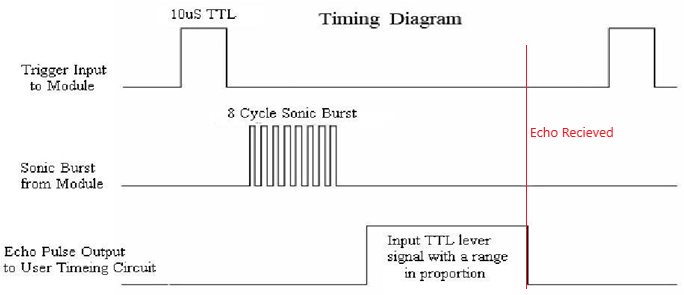
\includegraphics[width=0.5\textwidth]{./Figures/SonicSens_Timing.png}
\caption{Timing diagram for ultrasonic sensor\cite{Design_SonicSens}}
\label{fig:sonicsen_timing}	
\end{figure}

The ultrasonic sensor determines the range of an object that it is pointed at by sending out a set of 8 sonic pulses at \SI{40}{\kilo\hertz} when triggered \cite{Design_SonicSens}.  Once the set of pulse is sent the output is set to high until the sensor detects the return of pulse, at which point it drives the output low. With a regular interval trigger this results in a PWM output signal where the duty cycle corresponds to the distance between the sensor and the object it is facing. This distance is determined by using the speed of sound through air and half the time it takes for the echo to come back as shown in Equation: \ref{eqn:sonicsesns_lit_dist} \cite{Design_SonicSens}.

\begin{align}\label{eqn:sonicsesns_lit_dist}
Distance & = \frac{OutputHighTime \cdot SpeedOfSound}{2}
\end{align}

\newpage
\subsection{Converting PWM signals to analogue signals}
A PWM signal can be treated as the sum of a DC signal and a square-wave of equivalent duty cycle, as shown in Figure: \ref{fig:sonicsen_pwm}. Converting a PWM signal to its Fourier series equivalent shows that this DC component is equal to the amplitude of the PWM signal multiplied with the duty cycle\cite{Design_SonicSens_Filter}.

The core concept behind getting a analogue signal from a PWM signal is to use a low pass filter to remove the higher frequency components and leave the DC component \cite{Design_SonicSens_Filter}. The frequency of the PWM signal determines the frequency of the first harmonic as this harmonic will occur at the same frequency of the PWM signal.

Since it is impossible to physically realise a idea low pass filter the cut-off frequency must be set lower than the frequency of the PWM signal. This results in a trade of between the attenuation of the ripple voltage caused by the first harmonic of the PWM signal and the frequency at which the duty cycle of the PWM signal can be varied \cite{Design_SonicSens_Filter}. Increasing the order of the filter result in a better approximation of ideal low pass filter and allows for the cut-off frequency to be increased without sacrificing attenuation of the first harmonic.

\begin{figure}[H]
\centering
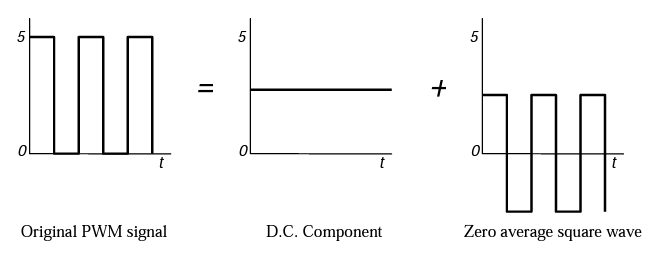
\includegraphics[width=0.5\textwidth]{./Figures/SonicSens_PWM.png}
\caption{Decomposition of a PWM signal\cite{Design_SonicSens_Filter}.}
\label{fig:sonicsen_pwm}	
\end{figure}

\newpage

\subsection{Digital to analogue converter opamp}
A summing amplifier works by combining several voltage inputs into one signal with no interference \cite{Lit_SumAmp}. The most common summing amplifier configuration is the inverting summing amplifier shown in Figure: \ref{subfig:inv_sum_amp}. This configuration makes the inverting node ideal for summing voltages as the non-inverting node is connected to ground the inverting node is now "virtual ground" \cite{Lit_SumAmp}. The gain for each input is given by the ratio between the feedback resistor and the input resistor.
\medskip\\
A non-inverting summing amplifier is similar to the inverting one however the inputs are connected to the positive terminal of the opamp as shown in Figure: \ref{subfig:noninv_sum_amp}. What makes this configuration less common is the fact that all inputs have an effect on all other inputs, this is due to the lack of "virtual ground" as seen in the inverting case \cite{Lit_SumAmp}. The advantages of a non-inverting configuration are that the input impedance is much higher than the inverting case and that the input summing part of the circuit is not affected by the changes to the amplifier's closed loop gain \cite{Lit_SumAmp_ET}.
\medskip\\
Common mode voltage range is based on the rail voltages supplied to the op amp but the specifics vary from op amp to op amp. Non-inverting op amps with the positive input terminal connected to ground don't have to consider common mode voltage however if the op amp has a offset at this terminal or is in a non-inverting configuration the common mode voltage gain will restrict what inputs result in a linear output. Since the common mode range is based on the rail voltage to increase the input range the rail voltages should be increased.
\medskip\\
Since the source for the binary signals are unideal they will have small output impedances, these sources typically can't drive high current. So in order to have most of the voltage drop occur across the summing circuit, the input impedance at the input terminals should be high.

Op amps are unable to source infinite current so if the receiving circuit has too low of an input impedance the op amp won't be able to sustain the desired voltage output. 


\begin{figure}[H]
\footnotesize
\centering
\begin{subfigure}[]{0.35\textwidth}
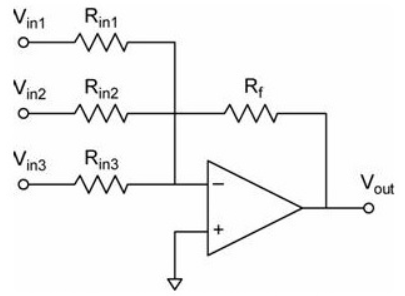
\includegraphics[width=\linewidth]{./Figures/DAC_InvAmp.png}
\caption{Circuit diagram for an inverting summing amplifier \cite{Lit_SumAmp}.}
\label{subfig:inv_sum_amp}	
\end{subfigure}
\begin{subfigure}[]{0.35\textwidth}
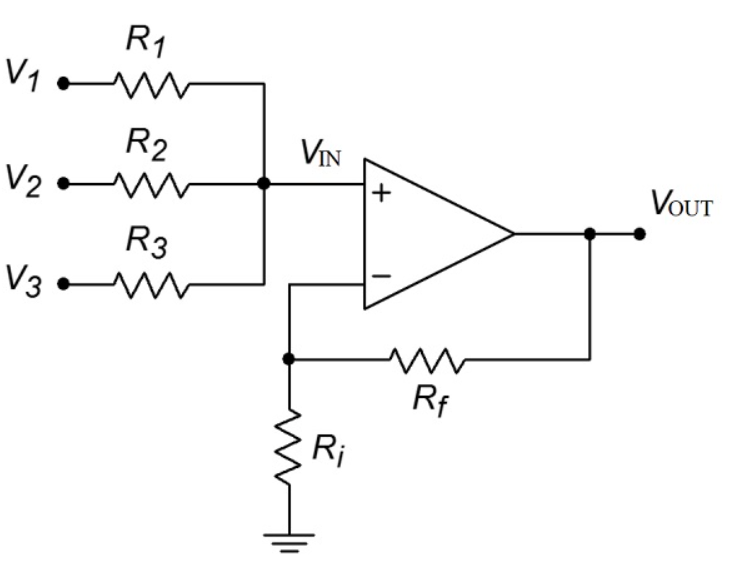
\includegraphics[width=\linewidth]{./Figures/DAC_NonInvAmp.png}
\caption{Circuit diagram for a non-inverting summing amplifier \cite{Lit_SumAmp}.}
\label{subfig:noninv_sum_amp}	
\end{subfigure}
\caption {Circuit diagrams of 2 summing opamp configurations}.
\label{fig:circuit_diagram}
\end{figure}
